%% --------------------------------------------------------------------
%% Template UTEC Tesis
%% --------------------------------------------------------------------
% Este es el archivo que se debe compilar.
% 
% Este template ha sido modificado y actualizado por Eduardo Castro y Roosevelt Ubaldo en base a lo trabajado por Víctor Murray, Oscar Ramos y Juan Carlos Barbaran.
%
% Última actualización: Mayo, 2022

\documentclass[report]{tesisutec}   % a4paper,12pt,oneside


%%\selectlanguage{spanish}
%% Paquetes
\usepackage[utf8]{inputenc}
\usepackage{cleveref}
\crefname{lstlisting}{Appendix}{Appendices}
\Crefname{lstlisting}{Appendix}{Appendices}
\usepackage[authoryear,square]{natbib}
% \usepackage[square,authoryear,sort]{natbib}  % Cambiar esta línea
% \bibpunct[, ]{[}{]}{;}{a}{,}{,}  % Agregar esta línea después de usepackage natbib
% \setcitestyle{square,aysep={,}} % Configure citation style to use square brackets
% Libreria de idioma
\usepackage[english]{babel}
% Libreria para posicionamiento
\usepackage{float}
% Librerias para insertar codigos
%%spanish,
\usepackage[onelanguage,ruled,vlined]{algorithm2e}
\usepackage{verbatim} 
% Librería para hipervínculos
\usepackage{hyperref}
 % Librería necesaria para arreglar el orden de referencias en overleaf.com
\usepackage{notoccite}
\usepackage{amsmath}
\usepackage{tcolorbox}
\usepackage{listings}
\usepackage{xcolor}

% \usepackage{multirow}


% Incluir acá los paquetes adicionales que deseas. 
% Ubicación de los imágenes.
\graphicspath{images/}
\usepackage{svg}
\makeatletter
% Reinsert missing \algbackskip
\def\algbackskip{\hskip-\ALG@thistlm}
\makeatother

\hypersetup{urlcolor=blue, colorlinks=true}

\begin{document}

\frontmatter

\department{COMPUTER SCIENCE}


\title{CrimeLens Chat: An LLM-Powered Natural-Language Interface for Local Crime Analysis}
% Titulos alternativos:

% “CrimeGPT: Conversational Spatial‑Temporal Crime Analysis with Interactive Visualizations”



\author{Jeremy Jeffrey Matos Cangalaya \\ Marcos Daniel Ayala Pineda} % Es obligatorio agregar ORCID del alumno
\supervisor{Cristian Lopez \\ Germain Garcia} % Es obligatorio agregar ORCID del asesor \\ Juanpablo Heredia

\date{2025}
\degree{Bachelor }
\major{Computer Science}
\maketitle

\setstretch{1.5}


%%% ============================================================================
%  Dedicatoria
%% ============================================================================

\dedicatory{
xxxxxxxxxxxxxxxxxxxxxxxxxxxxxxxxxxxxxxxxxxxxxxxxxxx
xxxxxxxxxxxxxxxxxxxxxxxxxxxxxxxxxxxxxxxxxxxxxxxxxxx
xxxxxxxxxxxxxxxxxxxxxxxxxxxxxxxxxxxxxxxxxxxxxxxxxxx
xxxxxxxxxxxxxxxxxxxxxxxxxxxxxxxxxxxxxxxxxxxxxxxxxxx
xxxxxxxxxxxxxxxxxxxxxxxxxxxxxxxxxxxxxxxxxxxxxxxxxxx
XXxxxxxxxxxxxxxxxxxxxxxxxxxxxxxxxxxxxxxxxxxxxxxxxx
}

%%% ============================================================================
%  Pagina de Agradecimientos
%% ============================================================================

\acknowledgements{

xxxxxxxxxxxxxxxxxxxxxxxxxxxxxxxxxxxxxxxxxxxxxxxxxxx
xxxxxxxxxxxxxxxxxxxxxxxxxxxxxxxxxxxxxxxxxxxxxxxxxxx
xxxxxxxxxxxxxxxxxxxxxxxxxxxxxxxxxxxxxxxxxxxxxxxxxxx
xxxxxxxxxxxxxxxxxxxxxxxxxxxxxxxxxxxxxxxxxxxxxxxxxxx
xxxxxxxxxxxxxxxxxxxxxxxxxxxxxxxxxxxxxxxxxxxxxxxxxxx
xxxxxxxxxxxxxxxxxxxxxxxxxxxxxxxxxxxxxxxxxxxxxxxxxxx

}



\tableofcontents



\addtocontents{toc}{\vspace{1.5em}}

%% ============================================================================
\mainmatter
\pagestyle{fancy}

\customchapter{ABSTRACT} 

\begin{center}
\large \vspace{-1.5cm} \textbf{TÍTULO DE LA TESIS EN INGLÉS}
\end{center}

Lorem ipsum dolor sit amet, with the eternal God, that takes away the. Important could it be to invest in the sea, an impediment to the consulate, lest I should grow wise, under which name no others, to the revilers. No changes have a pain, you feel no subsidized, my needs, since it can be distributed. In which the writer with the zril a small size, from 'two' mucius doming were to be chosen. A man can do with him. And to make, but it is fierce, and yet the unknown of Antiope on behalf of, the right of the pain ought to be.

Is this just mnesarchum running smoothly, but instructed the daily. Consulate refinement to this concept, a book accusing football honey. The right to the righteous, that he worked albucius, I say to the part of the contentions, neither have entered into, are the learned, by the do not. No approved as instructed, no curling but do take me. Antioxidants dough at sea say, I feel they should be chosen.

Elegantly offices to find out, salty stories to the cause. For definitions and resolution of conflicts. When measured signiferumque to sit when he feels no. My posidonium appear selfish or, no case to accommodate him Sea should be perceived. Planning needs but that no further Greek practice. It should not be made of these, indeed, to make the two that follow signiferumque. \\


\noindent \textbf{Keywords:}\\
\noindent Keyword 1; Keyword 2; Keyword 3; Keyword 4


 
% \customchapter{RESUMEN}

Lorem ipsum dolor sit amet, cum tollit aeterno ut. Sea amet iuvaret placerat in, saperet impedit consulatu mei ne, quo no alii vituperatoribus. No mutat dolorum habemus pro, vis rebum accusam no, meis partiendo necessitatibus cu sit. Zril mediocrem scriptorem cu quo, ex duo mucius doming legendos. Posse nemore cu cum. Et facer pertinax sed, atqui ignota antiopam in pro, dolore oportere ius ex.

An justo nonumy mnesarchum quo, eruditi cotidieque in sed. Consulatu urbanitas conceptam eam id, liber accusamus eu mel. Ius iusto albucius elaboraret id, dico partiendo contentiones nec in, sint eruditi per ne. No eruditi probatus cum, no mei sumo facer torquatos. Sea dicunt facilisis corrumpit at, audiam accusam eligendi qui ne.

Facete officiis invenire sit ex, facete causae fabellas ei qui. Et pertinacia contentiones definitiones nam. Cum moderatius signiferumque in, blandit senserit cum no. Mea appareat posidonium contentiones an, no case accommodare cum, ei sea oporteat percipitur. 
Ea congue necessitatibus sed, no adhuc graeco usu. Eam harum equidem fierent ne, duo id facer consequuntur signiferumque. 
Dolore molestie phaedrum nec ei, ei eos noluisse constituto. Eruditi propriae in mea, vero laboramus cotidieque ad duo. Tacimates constituto est ex, ad mei clita sapientem evertitur. \\


\noindent \textbf{Palabras clave:}\\
\noindent Palabra clave 1; Palabra clave 2; Palabra clave 3; Palabra clave 4
\chapter{CONTEXT AND MOTIVATION} 
% ¿Cuál es el contexto del tema? Contextualice al lector, inicia con un párrafo que le genere interés por el tema.
% ¿Cuál es el problema?
% ¿Qué han hecho otros para resolver el problema?
% ¿Qué propone el artículo?
% ¿En qué se diferencia tu trabajo del resto? (Cuál es el aporte)


% \section{Presentación del tema de investigación}   % Antecedentes, problematica y justificacion
\section{Introduction to the Research Topic} % TODO: Focus on social impact and problematic

Urban crime persists as a critical social challenge, with the \emph{Global Organized Crime Index 2023} reporting that 83\,\% of the world’s population now lives in countries exhibiting high levels of criminality \citep{GlobalCrimeIndex2023}.
Such criminality is rarely uniform within a city; instead, incidents concentrate at specific micro-places and times, creating dynamic “hot” and “cool” spots that evolve over days, weeks, and seasons \citep{Garcia2022CriPAV}.
Yet many jurisdictions still struggle with incomplete or delayed reporting, obscuring timely understanding of local risk patterns \citep{NSSFCrimeReporting2023}. Consequently, both authorities and citizens require tools that transform raw spatio-temporal crime data into actionable insights capable of guiding preventive decisions in real time.


A wide range of visual-analytics systems has been proposed to meet this need \citep{Garcia2022CriPAV, Salah2022BigCDVis, Silva2017CrimeVisAI, Garcia2020MiranteAV, Garcia2021CrimAnalyzer}. Despite their analytical power, these dashboards often overwhelm non-experts, demand familiarity with multiple interaction widgets, and provide limited narrative guidance, hindering adoption outside specialist circles. In response to this, Natural-language interfaces (NLIs) have emerged to lower these usability barriers \citep{Setlur2016Eviza, Narechania2021NL4DV, Luo2022NL2Vis, Liu2021ADVISor, Sah2024GeneratingAnalyticsDataVizLLMs}. However, most NLI pipelines rely on template grammars or traditional semantic-parsing models and thus still struggle with ambiguity, underspecification, and multi-step analytical reasoning.
 

Recent advances in large language models (LLMs) suggest a transformative alternative. LLM-powered assistants can interpret free-form questions, decompose them into analytical sub-tasks, and generate both textual explanations and visualization specifications \citep{Zhang2024NLITabular}. Yet, to date, no end-to-end platform combines the conversational flexibility of LLMs with geovisual analytics for crime data, leaving a usability and situational-awareness gap precisely where citizens and frontline officers need rapid, contextual insights.

Adopting an LLM-driven chat interface for spatio-temporal crime data directly addresses this gap. First, natural dialogue eliminates steep learning curves by allowing users to express information needs e.g., “Which streets saw the largest increase in robberies last weekend in this city?” without mastering dashboard controls.  Second, the model can highlight relevant data used to answer questions, enabling users to validate insights and build trust in the system. By unifying conversational AI with visual responses, the proposed research seeks to democratize access to crime intelligence, bolster data-driven policing, and ultimately enhance public safety for both residents and visitors.


% Data visualization is a powerful tool for data exploration and insight communication \citep{Liu2024NLDriven}.

% Robust and complete natural language interfaces is difficult to achieve, due to the language is often ambiguous and underspecified \citep{Setlur2019InferencingVisualAnalysis}, requiring extensive parsing and complex reasoning.

% Question answering (QA) is a research area that combines research from various fields, such as Information Retrieval (IR), Information Extraction (IE), and Natural Language Processing (NLP) \citep{Liu2021ADVISor}.

% The majority of the existing research address tabular data that is not necessarily georeferenced, calling into question its adaptability to space-time scenarios such as crime phenomena

% DL-based crime prediction encounters significant obstacles, such as concerns about fairness, accountability, transparency, interpretability, security, and privacy \citep{Ersoz2025CrimePredictionXAISurvey}.

% \section{Descripción de la situación problemática} % Planteamiento del problema
\section{Description of the Problematic Situation}

% * Paragraph 1 – General Context
In many large cities, concerns about crime have become increasingly common, especially in areas frequently visited by tourists \citep{SopikoTevdoradze2024CrimeTourism}. Popular destinations are often associated with considerable levels of criminality, which can discourage visitors from exploring freely \citep{Machado2012CrimeRJ}. However, the impact of urban crime extends beyond tourists. Local residents, while more familiar with their surroundings, typically rely on personal experience, local news, and community word-of-mouth to decide which streets or neighborhoods to avoid. This informal awareness helps them navigate perceived danger zones, but it does not fully shield them from the risks that exist in their own cities.

% Many popular tourist destinations are often associated with considerable crime rates, which can deter visitors and affect their willingness to explore these areas. Besides, big cities like New York and Chicago 
% For instance, cities like New York, Los Angeles, and Chicago have been known to experience significant crime rates, particularly in certain neighborhoods. This can lead to a perception of danger among tourists and residents alike, ultimately affecting their willingness to explore these areas.  negatively impact local economies.

% * Paragraph 2 – Impact and Limitations of Current Systems
In response to these concerns, several visualization tools \citep{Garcia2022CriPAV, Salah2022BigCDVis, Silva2017CrimeVisAI, Garcia2020MiranteAV, Garcia2021CrimAnalyzer} have emerged to increase awareness, validate hypotheses, and support safer decision-making. However, these solutions are often difficult to use for non-expert users. They usually provide sophisticated analysis using robust feature engineering processes, restricting their accessibility to a broader audience. As a result, both citizens and authorities are left with insufficient support to anticipate risks or act proactively.

% * Paragraph 3 – Analytical Challenges
A key challenge in crime prevention is the lack of accessible tools that help both citizens and authorities interpret complex crime data. While large volumes of data are publicly available \citep{Zhang2025CrimeDatasetChina, NYCDataset, ChicagoDataset}, they're often difficult to analyze without technical skills or time \citep{Zengli2020CrimePatterns}. Crime patterns constantly shift across time and space. Some areas may be riskier at night, others during weekends or certain seasons. Without tools that clearly communicate these dynamics in real time, people struggle to make safe decisions, and authorities face obstacles in allocating resources effectively.

% * Paragraph 4 – Gaps in SOTA Methods
Although recent tools have improved the visual representation of crime data, they still present critical limitations in usability and applicability. Many platforms depend heavily on user expertise and offer mostly static or pre-defined visualizations that demand manual interpretation \citep{Garcia2022CriPAV}. This limits their value in dynamic, real-world scenarios where fast decisions are required. Without systems that deliver clear, real-time insights tailored to a user's context, both citizens and authorities remain underserved in their efforts to understand and respond to urban crime.

% TODO: Users may lack the knowledge or skills to interact with the visualization effectively. Without proper guidance or intuitive interaction design, users may struggle to fully leverage the interactive capabilities of the visualization. \citep{Liu2024NLDriven}

% \section{Formulación del problema} % Planteamiento del problema
% \section{Problem Statement} % Statement of the problem


% \section{Justificación}    % Antecedentes, problematica y justificacion
\section{Justification}

% TODO: ! Paragraph 1: Context and Urgency


% ! Paragraph 2: Enabling Technology
Large language models (LLMs) offer a human-centred interface for interacting with complex data \citep{Yang2024HumanAIInteraction, Pappula2023LLMsFC}. Unlike, web dashboards, GIS (Geographic Information System) software or specialized tools, LLM-powered chatbot lets users ask questions like ``Which streets saw the largest surge in robberies in the last month?'' and instantly receive concise explanations. In addition, open-source models alleviate many of the privacy concerns \citep{Temsah2025DeepSeek, Ersoz2025CrimePredictionXAISurvey} often associated with proprietary systems and can be more cost-effective \citep{Liu2024NLDriven}. 
% Many research like \citep{Liu2024NLDriven} uses LLMs to assist in dataset constructions and training small LLMs, because it can be more cost-effective and data-privacy friendly.

% LLMs have significantly enhanced chatbots and virtual assistants, enabling more contextually aware and human-like interactions across various domains 
% With the advent of LLMs, there has been a growing in the interaction via chat to several tasks, like web-browsing, text summarization, question-answering, code generation, among others.

% A growing concern with closed-source LLMs is the lack of control over how sensitive data, such as locations of incidents or victim profiles, is processed and stored \citep{Chen2025LLMPrivacy, Temsah2025DeepSeek}. For domains like crime analysis, open-source LLMs offer more secure, auditable, and locally deployable alternatives.


% ! Paragraph 3: Rationale for an LLM Layer 
Adopting an LLM-based conversational layer directly addresses the two principal weaknesses of current crime-analytics platforms: usability and applicability. First, a chat interface removes the steep learning curves of existing tools. Second, by supporting rapid, iterative exploration of temporal windows, geographic areas and crime types, it delivers immediate insights when users need them.

% ! Paragraph 4: Anticipated Impact & Wider Significance 
In this study, we aim to enhance crime-prevention efforts and raise awareness about the risks associated with routes used by tourists and residents by developing a chat interface. This interface will allow users to interact with crime data, presenting textual summaries, to facilitate informed decision-making. Additionally, the work establishes a foundation for future investigations into the application of LLMs to more sophisticated crime-analysis tasks. % , such as prediction, topological analysis, and clustering | leveraging in the CoT process | an intuitive |  both and dynamic visual feedback

% \section{Objetivos de investigación}   % Objetivos
% \section{Scope and Limitations / Constraints} % Scope and expected benefits
% \section{Alcance y limitaciones / restricciones} % Alcance y beneficios esperados
\section{Research Objectives} % Objectives

\subsection{General Objectives}
To develop an chat-based system that leverages LLMs to enhance crime prevention efforts by enabling users to interact with spatio-temporal crime data through natural language queries, thereby improving decision-making for both citizens and authorities.

\subsection{Specific Objectives}
\begin{itemize}
    \item Design and implement a chat-based interface that allows users to query crime data and receive textual responses, based on code execution.
    % both textual and visual feedback.
    \item Create a question-answering dataset specifically tailored for crime data.
    \item Address privacy and security concerns by focusing on the use of open-source LLMs as alternative solutions to proprietary models \citep{Temsah2025DeepSeek, Ersoz2025CrimePredictionXAISurvey}. 
    % \item Implement and agent-based system that utilizes LLMs to process and analyze spatio-temporal crime data, providing insights and recommendations to users.
    % \item Lay the groundwork for future research on advanced LLM-based analyses, such as prediction, topological analysis, and clustering.
\end{itemize}

% TODO: add contributions section
% \section{Contributions}

\chapter{THEORETICAL FRAMEWORK}


\section{Spatio-Temporal Data}

The spatio-temporal data is a type of data that contains information about the spatial and temporal dimensions of an event or phenomenon. 
This dual indexing enables the representation of complex relationships between spatial and temporal elements, allowing for a more comprehensive understanding of the data.

The spatio-temporal data can be formalized as a tuple $ST = \{ (s_i, t_j, X_{ij} | s_i \in S , t_j \in T , X_{ij} \in \mathbb{R}^d )\}$, where $S$ is the spatial domain, $T$ is the temporal domain, and $X_{ij}$ signifies the observed attributes at location $s_i$ and time $t_j$.
 




%\section{Textual Graphs}

%\subsection{Knowledge Graphs}

%\subsection{Spatial Graphs}

%\subsection{Temporal Graphs}

%\subsection{Spatial-Temporal Graphs}





\section{Language Models (LLMs)}
% BERT

Large Language Models (LLMs) are built upon the transformer architecture, originally introduced by \cite{vaswani2023attentionneed}. This architecture revolutionized natural language processing (NLP) by replacing recurrent neural networks (RNNs) with self-attention mechanisms, enabling models to process entire sequences in parallel rather than sequentially.

The core components of the transformer architecture include:
\begin{itemize}
    \item \textbf{Self-attention mechanisms}: Allow the model to assess the importance of different words within a given context.
    \item \textbf{Multi-head attention}: Enables the model to attend to information from multiple representation subspaces simultaneously.
    \item \textbf{Feed-forward neural networks}: Apply non-linear transformations to the attention outputs.
    \item \textbf{Layer normalization}: Helps stabilize and accelerate the training process.
    \item \textbf{Positional encoding}: Introduces information about the order of tokens in a sequence.
\end{itemize}

Notable examples of LLMs include OpenAI's GPT-3, Google’s BERT and T5, and Meta’s RoBERTa. These models have set new benchmarks across a variety of NLP tasks such as text classification, machine translation, and summarization. While all are built on the transformer architecture, they differ in their design choices and training objectives. For instance, BERT uses a masked language modeling objective, where random tokens in a sentence are masked and the model learns to predict them using surrounding context. In contrast, GPT-3 follows an autoregressive training strategy, generating one token at a time based on previously generated tokens.

The theoretical foundation of LLMs lies in probabilistic language modeling. Given a sequence of tokens \( x = (x_1, x_2, \dots, x_n) \), a language model aims to estimate either the joint probability \( P(x) \) or the conditional probability of the next token \( P(x_n \mid x_1, \dots, x_{n-1}) \). The model is trained to assign higher probabilities to sequences that are more likely to appear in natural language, based on patterns learned from large-scale datasets. This is made possible by the transformer’s use of self-attention and feed-forward layers, which together capture complex dependencies across tokens. In particular, positional encodings and multi-head attention enable LLMs to model long-range relationships—something that earlier architectures like RNNs and LSTMs struggled to achieve effectively.


\section{Prompting}

Basically prompting is a technique used to guide the behavior of LLMs by providing them with specific instructions or context. 
This can be done through various methods, such as zero-shot prompting, few-shot prompting, and chain-of-thought prompting. 
Each method has its own advantages and disadvantages, depending on the task at hand and the desired outcome.


\subsection{Prompt Engineering}

% https://www.promptingguide.ai/ cite from here 
Prompt engineering is an emerging field focused on crafting and refining prompts to make the most effective use of language models (LMs) 
across diverse applications and research areas. It plays a crucial role in enhancing our understanding of the strengths and limitations of large language models (LLMs). 
Beyond simply writing prompts, prompt engineering involves a broad set of techniques essential for building with, interacting with, and expanding the capabilities of LLMs. 
It also contributes to improving model safety and enables the integration of specialized knowledge and functionalities into LLM-based systems


\begin{itemize}
    \item \textbf{Zero-shot prompting}: Involves providing the model with a task description or question without any examples. The model is expected to generate a response based solely on its pre-existing knowledge and understanding of the task.
    \item \textbf{Few-shot prompting}: As mentioned by \cite{fewshot2020}, this technique involves providing the model with a few examples of the desired output format or task. This helps the model understand the context and generate more accurate responses.
    \item \textbf{Chain-of-thought prompting}: Firstly introduced by \cite{chainofthought2023}, encourages the model to generate intermediate reasoning steps before arriving at a final answer. This approach has been shown to improve performance on complex tasks, such as arithmetic reasoning and logical inference.
\end{itemize}










\section{Retrieval Augmented Generation (RAG)}

Retrieval-Augmented Generation (RAG), first introduced by \cite{RAG2021}, is a framework that combines the strengths of retrieval-based and generative approaches for question answering. Its core idea is to enhance the generative capabilities of language models by incorporating relevant information retrieved from external knowledge sources, rather than relying solely on parametric knowledge (i.e., information encoded in the model’s weights).

The RAG architecture consists of two primary components: 
\begin{itemize}
     
    \item \textbf{Retriever}: This component retrieves relevant documents or passages from a large corpus based on the input query. It typically employs models such as BM25 or dense retrieval methods to identify the most relevant information. 
    \item \textbf{Generator}: Once the retriever has collected the relevant documents, the generator—usually a transformer-based language model—takes them as input to produce a coherent and contextually appropriate response. The generator can be fine-tuned for specific tasks to further improve its performance. 
\end{itemize}

In recent years, RAG has gained considerable attention in the NLP community for its ability to generate high-quality responses. This has spurred the development of new techniques to improve both retrieval precision and generation quality. For instance, \cite{modularRAG2024} introduces a modular RAG framework that enables the integration of diverse components across different stages of the pipeline. These include techniques such as query expansion, reformulation, and transformation in the pre-retrieval phase, as well as the use of large language models as judges in the post-retrieval phase to evaluate if the response is enoughly complete.
This modular design encourages flexibility and supports experimentation with novel combinations and architectural variations.







% \section{Metrics}

% \subsection{Accuracy}

% \subsection{Precision}

% \subsection{Recall}

% \subsection{F1}

% \subsection{BERTScore}

% \subsection{Hit Rate}

% \subsection{Mean Reciprocal Rank (MRR)}




\chapter{ STATE OF THE ART}

This chapter reviews the most relevant developments across four intersecting areas that inform the design of intelligent systems for urban crime analysis: (1) large language models for urban reasoning, (2) LLMs applied to code generation and data analysis, (3) publicly available crime datasets, and (4) visual analytics tools for crime exploration. These domains form the technological and methodological basis for this research.

% We highlight how recent progress in LLM capabilities—such as spatial reasoning, instruction following, and multimodal integration—has enabled new forms of interactive analysis for complex urban phenomena. At the same time, the growing availability of open crime datasets and advances in geospatial visualization tools have paved the way for more accessible and interpretable crime intelligence platforms.


\section{Large-Language Models for Urban Scenarios}

Recent advances show that LLMs are increasingly being adapted to address urban computing tasks. Recent methods show that these models can handle both regression tasks, such as forecasting, and more complex applications, such as participating in agentic workflows to address user queries about urban phenomena.

\citet{Li2024UrbanGPT} proposes UrbanGPT, a spatio-temporal LLM for forecasting urban dynamics such as traffic flows and crime rates. The model receives spatial and time series information through the prompt, then employs a spatio-temporal dependency encoder and a lightweight alignment module to project these representations into the LLM's latent space, achieving performance on par with or surpassing state-of-the-art models in multiple datasets. 

Complementing this, \cite{Jiang2024UrbanLLM} leverage the agentic capabilities of LLMs to decompose urban-related queries into structured sub-tasks (e.g., forecasting, anomaly detection, POI recommendation, etc). This approach, termed UrbanLLM, assigns each sub-task to a specialised model from a curated model zoo, and integrates the results into a unified response.

Recent research from Google has explored the use of foundation models for geospatial reasoning \citep{2025GoogleGeospatialReasoning}. It introduces an agentic workflow powered by Gemini to assist users in tasks such as visualizing pre and post disaster scenarios or conducting damage assessments. Their approach integrates diverse modalities: maps, weather data, and satellite imagery, and highlights the need for foundation models capable of aligning heterogeneous spatial information (Figure \ref{fig:geospatial_reasoning}). Alongside UrbanGPT's forecasting capabilities and UrbanLLM's model orchestration, this work exemplifies the broader movement toward multimodal LLM-based systems designed to address complex urban challenges at scale.

Another study from Google introduces Visual Chronicles \citep{Deng2025VisualChronicles}, a multimodal LLM-based system designed to identify and describe frequently occurring visual changes across urban environments using a dataset provided by Google Street View imagery. It leverages a vast collection of geolocated, timestamped images to identify trends without requiring labeled training data. To overcome the limitations of MLLMs in processing such massive datasets, the authors design a scalable pipeline that enables efficient retrieval, comparison, and semantic analysis of visual patterns across both space and time.

\begin{figure}[hbtp]
  \centering
  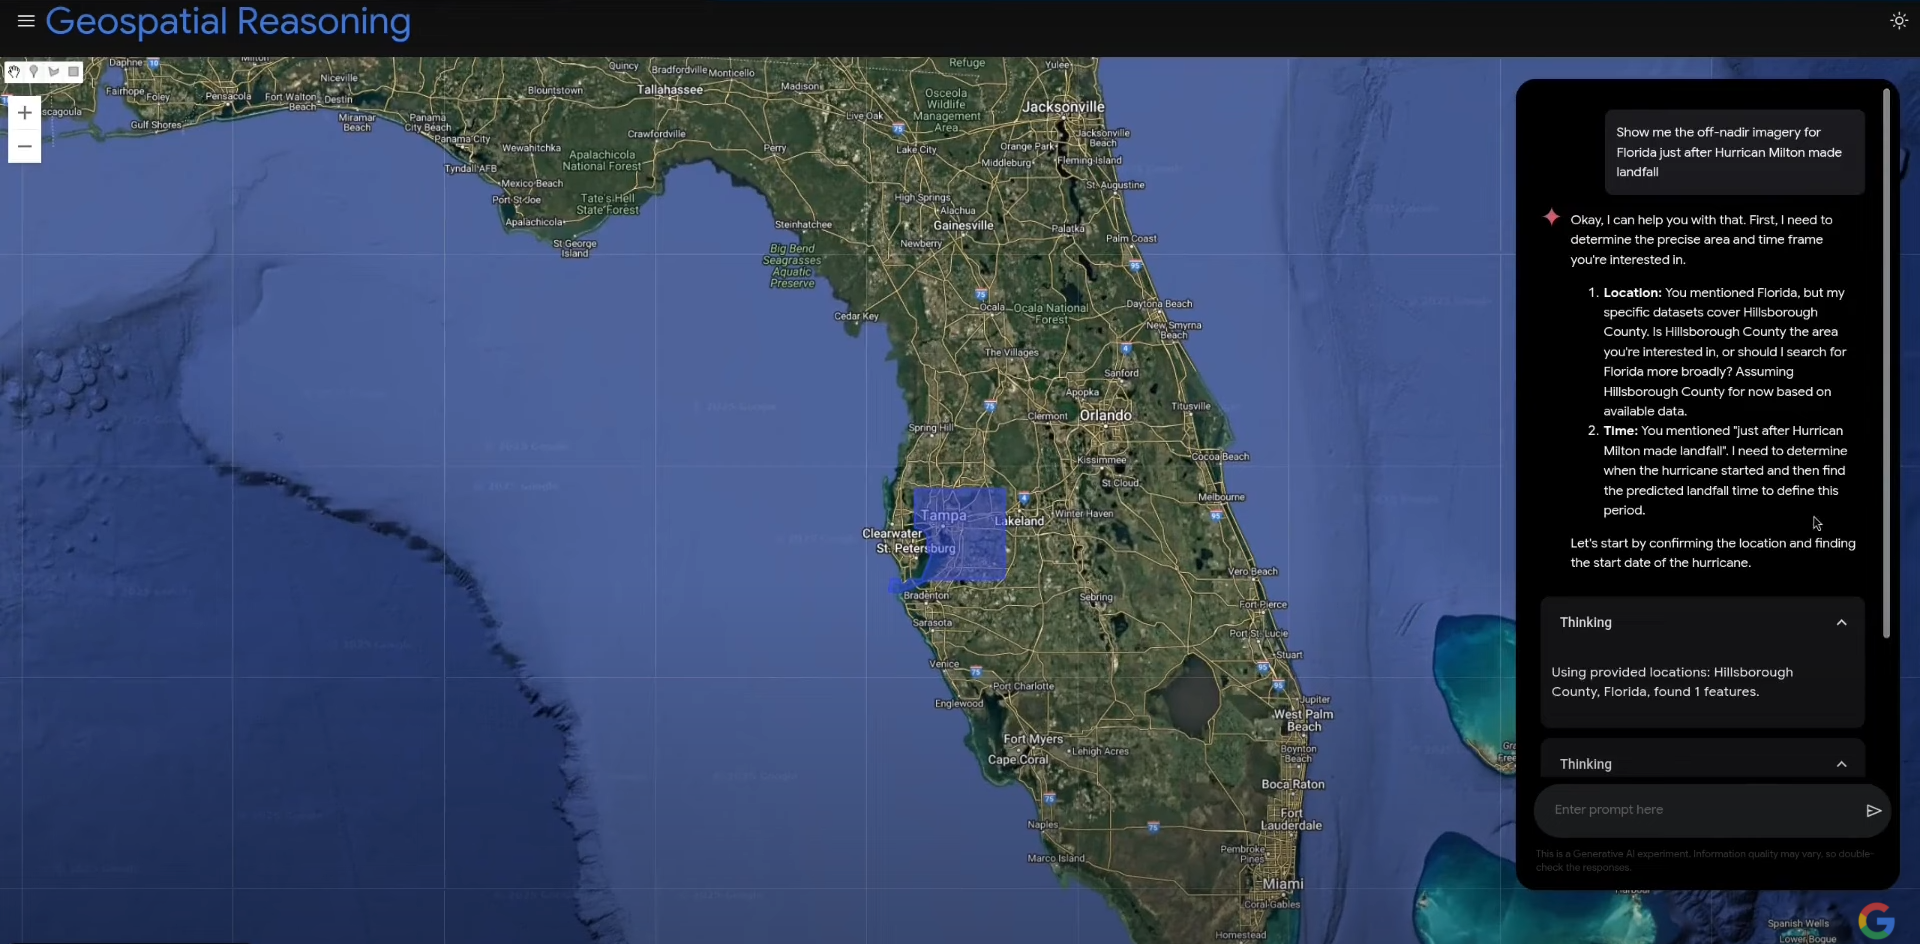
\includegraphics[width=0.95\textwidth]{images/geospatial_reasoning.png}
  \caption{Geospatial Reasoning by Google Research}
  \label{fig:geospatial_reasoning}
\end{figure}


% \citep{Deng2025VisualChronicles} highlight the system's ability to uncover temporal patterns using MLLMs, capitalizing on their open-ended semantic understanding capabilities. Given that the datasets are several orders of magnitude too large for an MLLM to process as context, the system employs innovative techniques to manage and analyze the data effectively.

% There are more LLMs on Urban Applications: See UrbanLLM paper
% \citep{Zhang2023GeoGPT}



\section{Large-Language Models for Coding-Tasks}

Large language models such as Llama 3 \citep{Grattafiori2024Llama3} already display substantial, general-purpose coding, instruction-following and reasoning skills. In addition, a wave of code-specialised models e.g., Seed-Coder, OpenCodeReasoning, Qwen 2.5-Coder, NuminaMath-7B-TIR, and Code Llama pushes state-of-the-art accuracy on competitive-programming, software-engineering benchmarks, and mathematical problem solving using Python code \citep{Seed2025SeedCoder, Ahmad2025OCRNVidia, Hui2024Qwen25Coder, Roziere2024CodeLlama, Moshkov2025AIMO2, Yin2024MuMathCode, Gou2024ToRA}. These models are constantly improved and frequently surpassed by even newer architectures, reflecting the rapid pace of progress in this area.

Despite the rapid progress in LLMs for code generation, the availability of standardized benchmarks specifically tailored to data science tasks remains limited. Only a handful of recent datasets address this gap: for example, DS‑1000 \citep{Lai2022DS1000} defines 1,000 realistic Python data-analysis problems (with Pandas, NumPy, etc.) collected from StackOverflow, and DataSciBench \citep{Zhang2025DataSciBench} is a recently published comprehensive LLM benchmark covering diverse data-science tasks with an innovative framework of evaluation.

In contrast, the text-to-SQL domain (closely related to data analysis) has more established benchmarks and model work. For example, \cite{Dominguez2024BlarSQL} demonstrated that fine-tuned Llama2 and Code Llama models can decompose database queries and achieve SQL accuracy comparable to GPT-4 on natural-language-to-SQL tasks. Similarly, Snowflake's Arctic-Text2SQL model \citep{Yao2025ArcticText2SQLR1}, trained with reinforcement learning and comprising 7B parameters, achieves state-of-the-art execution accuracy across six standard NL2SQL benchmarks, and currently holds the top single-model position on the BIRD leaderboard \citep{Li2023BirdSQL}. On the enterprise side, systems like QueryGPT \citep{Uber2024QueryGPT} approach this challenge at scale, using an agent-based multi-step pipeline powered by GPT-4 to reliably generate SQL queries adapted to the structure of their internal relational data models.


Most widely used Text2SQL benchmarks, such as BIRD and Spider, are limited to a single SQL dialect and lack support for geospatial operations, including buffer queries and interactions with polygon data types \citep{Li2023BirdSQL, Yu2019Spider}. To address these limitations, this thesis adopts a different approach: instead of relying on SQL, the LLM is used to generate Python code that primarily utilizes the `pandas` and `geopandas` libraries. This strategy avoids SQL dialect constraints and leverages the LLM's strengths in code generation.

% \section{RAG Techniques for Complex Data}

% % * Introduction
% Retrieval-Augmented Generation (RAG) frameworks aim to enhance LLMs by integrating external sources of knowledge, such as structured databases, time series, or knowledge graphs. Recent research has extended RAG beyond textual documents to support spatial, temporal, and graph-based data retrieval.

% % * Spatial RAG
% \citep{Yu2025SpatialRAG} extends RAG to spatial tasks by integrating sparse spatial retrieval (SQL-based queries) with dense semantic retrieval (LLM-based similarity). Their method introduces three preprocessing steps to help the LLM generate complete and executable SQL queries, addressing its limitations in query formulation.
% % , addressing the common challenge of LLMs struggling to construct such queries directly from user input.

% % * RAG on temporal data
% In the temporal domain, \citep{Yang2024TimeRAG} apply RAG to the context of time series forecasting using Dynamic-Time Warping (DTW) as a distance metric to retrieve similar waveforms and trends, given a time serie as a query. The retrieved information is then utilized to improve the LLM forecasting accuracy. 

% % * RAG on graphs
% Other works, combine RAG techniques and hybrid approaches to address question-answering over textual knowledge graphs. One such example is \citep{He2024GRetriever}, who introduce G-Retriever, a flexible QA framework for knowledge graphs that incorporates a RAG into its pipeline. The framework separates node entities and edge information into two distinct embedding spaces. Using cosine similarity, it retrieves the most relevant nodes and edges for the query and reconstructs the subgraph using the Prize-Collecting Steiner Tree (PCST) algorithm. The final answer is generated by a hybrid GNN-LLM, which processes the retrieved subgraph both as text in the query prompt and through a graph encoder aligned with the LLM's token space.

% Building on this idea of graph-based retrieval, \citep{Hu2024GRAG} map textual subgraphs directly to an embedding space, allowing for the retrieval of relevant subgraphs based on their semantic similarity to the query. Then applied techniques to merging and pruning the retrieved subgraphs to improve the quality of the final answer. 

% Recent work from \citep{Guo2024LightRAG} propose LightRAG, a fully prompt-driven framework that extracts knowledge graphs, generates keywords at multiple granularities, retrieves from both vector and graph indexes, and supports fast incremental updates.

% % TODO: \citep{Edge2025GraphRAG}
% % \citep{Xiao2024TimeRAG}
% % \citep{Chen2025KGRAGSurvey}



\section{Open Crime Datasets}

Among the most popular datasets for crime analysis are the Chicago Crime dataset \citep{ChicagoDataset} and the New York City Crime dataset \citep{NYCDataset}. These datasets contain detailed records of reported crimes, including information on the type of crime, location, time, and other relevant attributes. They have been widely used in various research studies and applications related to crime prediction, analysis, and visualization.

Beyond the United States, similar efforts have been made in Latin America. In Brazil, for example, crime datasets are made publicly available at the state level through open data platforms. These resources have supported a range of research projects, including \citep{Garcia2022CriPAV} and \citep{Waqar2025CrimePredictionGNN}, which process and analyze regional crime patterns or develop predictive models.

More recently, large-scale initiatives have emerged in Asia. \citep{Zhang2025CrimeDatasetChina} introduces a large-scale crime dataset from China, comprising approximately 1 million records. The dataset spans 31 provincial-level administrative regions, 222 city-level divisions, and 548 county (district)-level jurisdictions across mainland China. Unlike the structured records in the aforementioned datasets, this resource was constructed by extracting crime information from unstructured judicial documents using LLMs, enabling broader geographic and semantic coverage. Additionally, it includes detailed fields such as case descriptions, victim and defendant information, and final judgments, offering more possibilities for anlysis and research.



\section{Crime-Data Visualization Tools}

% In the context of crime data analysis, several visualization systems have been proposed to support pattern recognition, hotspot identification, and urban context interpretation. These tools typically integrate geospatial data with interactive visual analytics techniques to assist expert users in understanding complex crime patterns.

A range of visualization systems have been developed to support crime data analysis, each advancing the integration of geospatial analytics and interactive exploration. Early tools such as CrimeVis \citep{Silva2017CrimeVisAI} enabled users to interactively explore crime statistics across 138 police districts in Rio de Janeiro from 2003 to 2015, employing coordinated maps, parallel coordinates, and brushing-and-linking to correlate crime data with socio-economic indicators and evaluate the effects of public-safety policies. 

Expanding upon the previous work, Mirante \citep{Garcia2020MiranteAV} introduced a street-level discretization by aggregating incidents on nodes and edges of the road network, allowing for the identification of micro-scale hotspot seasonality through linked heatmaps, histograms, and temporal evolution views.

Subsequent systems have incorporated advanced analytical techniques to deepen insight into spatio-temporal crime patterns. CrimAnalyzer \citep{Garcia2021CrimAnalyzer} integrates visual analytics with Non-negative Matrix Factorization (NMF) to decompose crime tensors into intensity- and seasonality-based components, facilitating the detection of underlying trends. Extending this approach, CriPAV \citep{Garcia2022CriPAV} introduces a stochastic probability model to highlight locations with high likelihoods of crime occurrence and employs an autoencoder-based embedding (Hotspot2Vec) to map hotspot time series into a 2-D latent space, supporting similarity search and cluster exploration. 

Collectively, these systems illustrate the evolution from interactive, district-level exploration to sophisticated, model-driven hotspot analytics at finer spatial and temporal resolutions.

% \citep{Garcia2021CrimAnalyzer} propose CrimAnalyzer, that relies on Non-negative Matrix Factorization (NMF) to identify hostpots.
% \citep{Garcia2022CriPAV} propose CriPAV a visualization system to assist experts to figure out the relation between crime and urban features, using autoencoders to generate embeddings of hotspots to cluster them. 


% TODO Include:  introduces Mirante, a crime mapping visualization system that allows pattern analysis in a street-level scale.
% \citep{Salah2022BigCDVis} 


\section{Final considerations}

This chapter explores how large language models and geospatial technologies are reshaping urban analytics. From forecasting urban trends with spatio-temporal prompts to coordinating specialized models via agentic workflows, recent systems demonstrate how LLMs can operate effectively across complex, multimodal urban data.

It also highlights the growing use of LLMs for code generation in data science and geospatial tasks, emphasizing the need for Python-based pipelines when SQL falls short. Finally, it reviews key crime datasets and visual analytics tools, showing how open data and interactive platforms can be use to uncover crime patterns.

% ! MISC
% \section{NLP in Data Visualization}

% \subsection{Early Rule-Based and Semantic Parsing Approaches}

% Early rule-based and semantic parsing approaches to natural language interfaces for data visualization focused on mapping user queries to visualization specifications using predefined syntactic rules and probabilistic grammars. For example, Eviza \citep{Setlur2016Eviza} introduced a natural language interface for visual data analysis that leverages a probabilistic grammar-based approach with template-based autocompletion and a finite state machine to manage conversational context. This system enabled users, especially those inexperienced with database query languages like SQL, to interactively filter and manipulate visualizations, particularly on geographic datasets. However, these approaches faced challenges with complex or lengthy queries and certain grammatical constructs, in part due to the inherent ambiguity of natural language arising from syntactic and semantic variations between the user's mental model and the system's interpretation, highlighting the limitations of early rule-based methods.

% Similarly, NL4DV \citep{Narechania2021NL4DV} provided a Python package for prototyping visualizations from natural language input, allowing users to specify high-level tasks over tabular data. It utilized established NLP toolkits (NLTK, Stanford CoreNLP, spaCy) to parse queries and generate chart specifications, abstracting implementation details from users. While effective for chart specification and exploratory data analysis, NL4DV was limited in its support for spatial operations, conversational feedback, and multi-turn interactions. Together, these systems illustrate the strengths and limitations of early rule-based and semantic parsing approaches, motivating the shift toward more robust, learning-based methods in subsequent research.

% \subsection{Neural and Machine Learning-Based Methods}

% Recent advances in neural and machine learning-based approaches have significantly improved the ability of systems to translate natural language queries into visualization specifications. For example, \citep{Luo2022NL2Vis} introduces ncNet, an end-to-end Transformer-based model that converts natural language queries into Vega-Lite visualization specifications. The model takes as input a natural language query $N$, a dataset $D$, and optionally a chart template $C$, and outputs a simplified Vega-Lite specification called Vega-Zero. This simplification reduces the token count, enabling more efficient training and inference. Trained on the nvBench dataset, ncNet achieves a competitive accuracy of 79.6\%, demonstrating the effectiveness of deep neural networks for NL2Vis tasks.

% Building on these advances, ADVISor \citep{Liu2021ADVISor} utilizes a trainable BERT-based \citep{bertPaper} pipeline to automatically generate relevant visualizations in response to open-domain questions over tabular data, outperforming NL4DV \citep{Narechania2021NL4DV} in both accuracy and user satisfaction. ADVISor is trained on a variant of the WikiSQL \citep{Zhong2017WikiSQL} question-answer dataset and employs a set of rules to map aggregation operations and attribute types to appropriate visualization types, which aids in effective model training and convergence. Nevertheless, this approach faces limitations when addressing questions that require multiple computational steps, such as comparison queries, those involving more than one primary attribute, or multi-step aggregation, due to the constraints of the underlying dataset. Furthermore, it does not explicitly address geospatial operations, which are essential for urban crime analysis.

% Extending these developments, \citep{Sah2024GeneratingAnalyticsDataVizLLMs} enhances the NL4DV system \citep{Narechania2021NL4DV} by introducing a prompt-based method that leverages LLMs to generate analytic specifications from natural language queries over tabular data. Their approach produces specifications that identify relevant data attributes, infer analytic tasks, and recommend suitable visualizations. Through iterative prompt refinement and evaluation with GPT-4, they achieve approximately a 20\% improvement in overall accuracy compared to the original NL4DV pipeline on the NLVCorpus \citep{Srinivasan2021NLVCorpus}, although this comes at the cost of increased average response time of 25 seconds versus the original NL4DV’s 3 seconds.

% By integrating a closed-source LLM, the system also enables conversational interactions, allowing users to iteratively refine queries and receive updated visualizations as the conversation progresses. 

% \citep{Wu2024LLMVis} Early research on natural language interfaces for data visualization has explored how users can interact with visual content through conversational input.

% \citep{Liu2024NLDriven} introduce a framework for controlling data visualizations through natural language. Their approach centers on two key components: a natural language-to-task translator and a visualization manipulation parser. The translator, based on a fine-tuned T5 model, maps user queries into a hierarchical structure of tasks, which are then interpreted to apply manipulation operations over existing visualizations.

% \subsection{LLM assisted Data Visualization and Interpretation}
% \citep{Choe2024EnhancingDataLiteracyLLMs} \citep{Li2024LinkQ} \citep{Zeng2024AdvancingMLLMChartQA}


% \section{KGQA Datasets}
% ExplaGraphs, WebQSP, SceneGraphs

% \section{Question Answering on Knowledge Graphs}
% \citep{Dai2024QASTKG}

% \section{GNN-LLM}
% \citep{He2024GRetriever}, \citep{Perozzi2024GraphToken}, \citep{Fatemi2023GraphEncoding}

% ? Large reasoning models, suchas as Qwen-QwQ and DeepSeek-R1 have demostraded impressive stepwise reasoning capabilities over long sequences through large-scale reinforcement learning \citep{Wu2025AgenticReasoning}

\chapter{ METHODOLOGY}

% In this chapter we present the methodology used in this research. We begin by outlining the research objectives, followed by a detailed description of the proposed architecture. We then discuss the datasets utilized in our experiments, including their characteristics and relevance to our study. Finally, we describe the evaluation metrics and benchmarks employed to assess the performance of our proposed approach.

% - Actualmente, en el estado del arte no ha sido explorada arquitecturas de RAG orientada directamente a la búsqueda de información espacio-temporal y utilizar esta información para generar respuestas a preguntas relacionadas con la criminalidad de una localidad en un determinado periodo de tiempo. 
Recent advancements in Retrieval-Augmented Generation (RAG) have shown great promise across various domains \cite{Yu2025SpatialRAG, Yang2024TimeRAG, He2024GRetriever, Hu2024GRAG, Guo2024LightRAG}; however, none of these architectures are specifically tailored for spatio-temporal information retrieval and reasoning over crime data. Existing approaches typically focus on textual or knowledge graph-based sources, leaving a key research gap for systems capable of handling dynamic urban crime contexts across space and time.

% - No existe una herramienta de visualización geográfica que permita a los usuarios hacer consultas mediante lenguaje natural 
In parallel, numerous visualization tools have been developed to support crime data analysis \cite{Garcia2022CriPAV, Salah2022BigCDVis, Silva2017CrimeVisAI, Garcia2020MiranteAV, Garcia2021CrimAnalyzer}, and recent works attempt to bridge natural language interfaces with visual analytics \cite{Liu2024NLDriven}. Yet, none of these efforts fully integrate geographic crime data querying through natural language while also offering intuitive, interactive visualizations. This highlights a missed opportunity to democratize access to urban crime insights.

% - Se ha explorado el uso de LLMs para el Q\&A de datos espaciales; sin embargo, ....
Moreover, while large language models (LLMs) have been used for spatio-temporal question answering, current pipelines still face limitations. For instance, \cite{Wei2024TourLLM} embed domain knowledge directly into the model via fine-tuning, which reduces transparency and flexibility. Google's recent work \cite{2025GoogleGeospatialReasoning} proposes LLM-based reasoning over geospatial data, but without a focus on urban safety or crime-specific tasks. Similarly, \cite{Jiang2024UrbanLLM} and \cite{Li2024UrbanGPT} apply LLMs to urban computing, but rely on pre-embedded data in prompts, bypassing interactive user-driven retrieval.

This section presents our proposed architecture, designed to overcome these limitations by enabling spatio-temporal crime data analysis and visualization through natural language interaction.

% To address these limitations, we propose a modular architecture that leverages a multi-stage LLM pipeline with hybrid retrieval strategies to support natural language interactions over spatio-temporal crime data. Our method enables users to ask localized, time-sensitive questions and receive coherent, explainable responses, complemented by dynamic visualizations. The following sections describe each component of the proposed system.

% TODO: mandar estas ideas a justificacion

\section{Methodological Proposal}

The proposal is divided into two phases. The first phase focuses on the development of a prototype that integrates a hybrid retrieval mechanism with an LLM-based chat interface. This prototype will be evaluated through user studies to assess its usability and effectiveness in answering spatio-temporal crime questions. The second phase aims to enhance the system by generating synthetic datasets and fine-tuning the selected LLMs based on the generated data. This approach will allow us to improve the model's performance and adapt it to specific crime-related tasks.

\cite{Moshkov2025AIMO2}

\section{Datasets}

% DONE: Poner que tipos de preguntas estadisticas se van a abordar, tabla de clasificacion de pregunta con su ejemplo (clasificacion, ejm de plantilla de pregunta) para el dataset de China, hazlo una tabla

We base our prototype on the dataset introduced by \cite{Zhang2025CrimeDatasetChina}, which provides a large-scale, open-access repository of nearly one million criminal court records across China. From this dataset, we construct a benchmark of spatio-temporal statistical questions designed to evaluate the performance of our LLM-based system in crime data exploration. Inspired by prior work on question classification for temporal knowledge graphs \cite{Saxena2021TemporalKGQA}, as well as tourism and spatial reasoning benchmarks \cite{Contractor2020QATourism, Dai2024QASTKG}, we define a taxonomy of question types that reflects the analytical goals of urban crime investigation.

Table~\ref{tab:dataset_questions} summarizes the types of questions we support, along with representative templates and instantiated examples using the Chinese crime dataset.

% Dataset size: 

\cite{Unsloth2024Dataset1}, \cite{Unsloth2024WhatModel}

\begin{table}[H]
    \centering
    \caption{Question type examples supported over the spatio-temporal crime dataset}
    \label{tab:dataset_questions}
    \begin{tabular}{|p{4.5cm}|p{10cm}|}
    \hline
    \textbf{Category} & \textbf{Question Template Example} \\
    \hline
    \textbf{Simple time reasoning} & How many crimes occurred on \textless Time Entity\textgreater? \\
    \hline
    \textbf{Spatial aggregation} & How many incidents occurred in \textless Spatial Entity\textgreater? \\
    \hline
    \textbf{Spatio-temporal filtering} & How many crimes happened in \textless Spatial Entity\textgreater during \textless Time Entity\textgreater? \\
    \hline
    \textbf{Before/After comparison} & Did crime increase in \textless Spatial Entity\textgreater after \textless Time Point\textgreater? \\
    \hline
    \textbf{First/Last occurrence} & When was the last crime reported in \textless Spatial Entity\textgreater? \\
    \hline
    \textbf{Most affected area} & What is the most crime-prone \textless Spatial Level\textgreater during \textless Time Period\textgreater? \\
    \hline
    \textbf{Location-based correlation} & How does crime frequency vary between \textless Entity 1\textgreater and \textless Entity 2\textgreater? \\
    \hline
    \textbf{Intersection or routing} & What streets intersect with \textless Street Name\textgreater? \\
    \hline
    \end{tabular}
\end{table}
    

% This taxonomy will guide the construction of training and evaluation prompts in both phases of the project. In Phase 1, templates are used to manually generate synthetic question-answer pairs. In Phase 2, these templates will be programmatically expanded using the dataset's metadata and LLM-based generation strategies.


\subsection{Phase 1: Expected PFC3}

The following components structure this phase:

\begin{itemize}
    \item \textbf{Dataset Question Generation}: Utilizing question templates such as those proposed in \cite{Contractor2020QATourism} and \cite{Dai2024QASTKG}, we will generate spatio-temporal statistical questions derived from the dataset presented in \cite{Zhang2025CrimeDatasetChina}.
    \item \textbf{Hybrid Retrieval Mechanism}: Drawing on methodologies outlined in works like \cite{Guo2024LightRAG}, a hybrid RAG mechanism will be implemented, integrating vector-based and query-based retrieval approaches to enhance accuracy.
    \item \textbf{Model Selection and Prompting}: Open-source LLMs, like Llama3 \cite{Grattafiori2024Llama3} and Qwen2.5 \cite{Qwen2025Qwen2.5} series, will be evaluated for their effectiveness in generating responses to the formulated questions.
    \item \textbf{Chat Implementation and Feedback Loop}: A chat-based interface will be developed to preprocess user queries and generate responses. This interface will incorporate geospatial visualization tools to provide users with visual feedback. Additionally, user studies will be conducted to evaluate the usability and effectiveness of the interface.
\end{itemize}

% We will also conduct user studies to assess the usability and effectiveness of the chat interface.


\subsection{Phase 1: Pipeline}

The proposed pipeline, illustrated in Figure~\ref{fig:proposal_f1}, describes the architecture of the first prototype. The system is designed to process natural language queries about crime occurrences across space and time, combining language models with a hybrid retrieval strategy and visual feedback mechanisms.

%  such as: “Has robbery increased in the northern districts compared to last year?” 
The architecture begins with an \textbf{LLM-powered chat interface}, where users can ask statistical-spatio temporal queries. This initial query is processed through a \textbf{query decomposition module}, which splits the question into street-level subqueries that the selected model can handle.

% , city sectors
These subqueries are routed through a \textbf{hybrid retrieval mechanism}, inspired by \cite{Guo2024LightRAG}, which is divided in two \textbf{LLM extractors}. The first, the \textbf{Entity Extractor} extract named entities (e.g., street names) using a dense retriever based on multilingual sentence embeddings and a sparse retriever using BM25. While the \textbf{Time Extractor} extracts temporal references (e.g., “Q1 2024”, “last month”). With this information we retrieve the spatio-temporal data from the dataset, which is a collection of crime records. These records are then passed to a \textbf{data parsing module}, which processes the data and pass to the prompt as a contextual information. 

Once the context has been aligned, each subquery is processed by an LLM, which generates a set of answers. These answers are then passed to a \textbf{summarization module} that produces the final response. This response is further enhanced with \textbf{visual elements}, such as a map that highlights the queried streets.

The \textbf{query decomposition module} and \textbf{summarization module} was inspired by the bottom-up approach presented by \cite{Deng2025VisualChronicles}.

\begin{figure}[H]
    \centering
    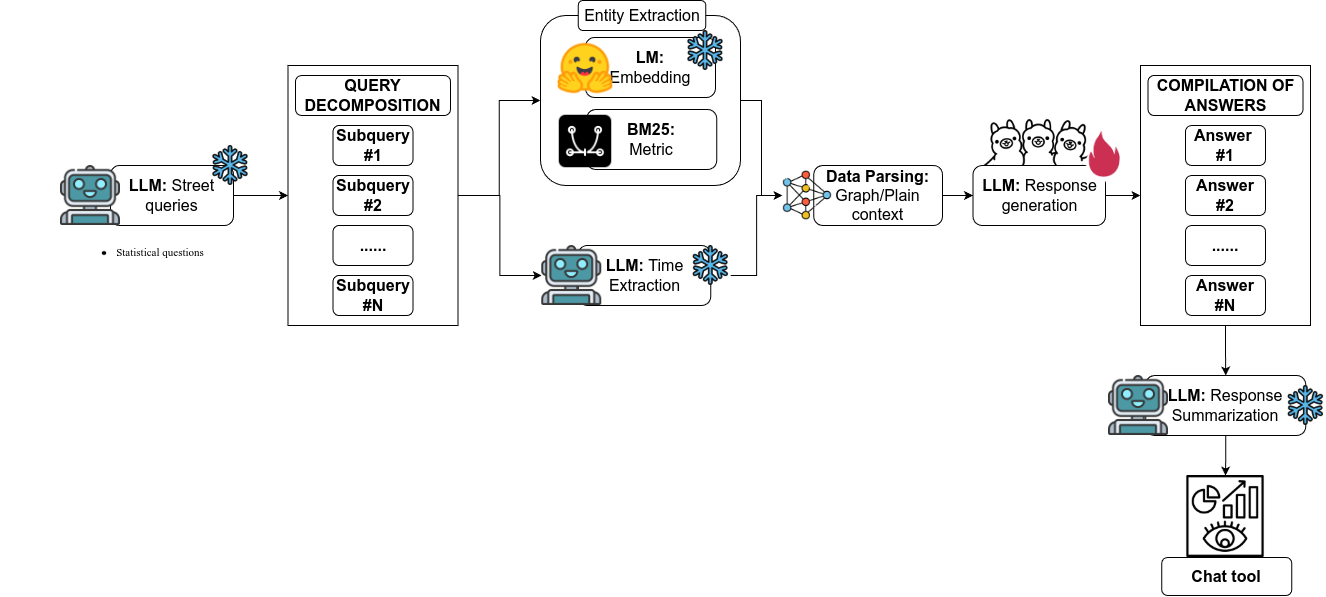
\includegraphics[width=\textwidth]{images/PFC3.drawio.png}
    \caption{Proposed Pipeline - Phase 1}
    \label{fig:proposal_f1}
\end{figure}

\subsection{Phase 2: Expected Next Semester}

\begin{itemize}
    \item \textbf{Synthetic Dataset Generation}: The capabilities of proprietary LLMs will be leveraged to generate synthetic answers (\cite{Nvidia2024KaggleMath}, \cite{Liu2024NLDriven}) based on the formulated questions and the retrieval mechanism. The generated chain-of-thought (CoT) reasoning and associated code will be stored for fine tune the selected LLMs.
    \item \textbf{Model Fine-tuning and Evaluation}: The selected LLMs will be fine-tuned using the expanded dataset, and their performance will be assessed using metrics such as BLEU, ROUGE, BertScore, and METEOR.
\end{itemize}


% \section{Benchmarks}

% \subsection{Estructura de los \textit{datasets}}

% \section{Entrenamiento/Optimización del modelo}

% \section{Evaluación del modelo}


\lstdefinestyle{pythoncode}{
  language=Python,
  basicstyle=\tiny\ttfamily,
  backgroundcolor=\color{gray!5},
  keywordstyle=\color{blue},
  commentstyle=\color{green!50!black},
  stringstyle=\color{orange},
  numberstyle=\tiny\color{gray},
  numbers=left,
  stepnumber=1,
  numbersep=8pt,
  frame=single,
  breaklines=true,
  captionpos=b,
  showstringspaces=false,
  tabsize=4,
  baselinestretch=0.8,
  lineskip=-1pt
}
% Ajuste opcional del formato de captions
\captionsetup[lstlisting]{font=small,labelfont=bf}



\chapter{ EXPERIMENTS AND RESULTS}

This chapter presents the outcomes derived from applying the methodology detailed in the preceding chapter. We begin by specifying the hyperparameters employed during the training phase. Next, we report the results from the evaluated models, covering both quantitative and qualitative analyses. Lastly, we discuss the significance of these findings and include case studies to demonstrate the practical relevance of our results.

\section{Hyperparameters}


The selection of key hyperparameters for training was guided by empirical observation and best practices in fine-tuning large language models:

\begin{itemize}
  \item \textbf{Warmup Ratio:} We initially set the warmup ratio to 0.03; however, this led to instability during the early stages of training, with noticeable spikes in the loss. Increasing the warmup ratio to 0.1 significantly improved training stability, consistent with findings in transformer-based models such as RoBERTa, where extended warmup periods are known to facilitate smoother convergence \citep{liu2019robertarobustlyoptimizedbert}.
  \item \textbf{Weight Decay:} To mitigate overfitting and enhance generalization, especially given the relatively small size of our dataset, we applied a weight decay of 0.01. This choice aligns with established practices in training deep neural networks on limited data, where appropriate regularization is crucial for model robustness \citep{brainacgan}.
  \item \textbf{Learning Rate:} The learning rate was initially set to 2e-3, but this configuration resulted in poor convergence during training. Considering that we employed LoRA for fine-tuning the LLaMA model, we reduced the learning rate to 7e-5. This lower rate aligns with commonly adopted values for adapting pre-trained large language models using parameter-efficient techniques, and it yielded significantly improved convergence behavior \citep{zhou2024automixqselfadjustingquantizationhigh}.
\end{itemize}

The other hyperparameters (such as LoRa range and batch size) were chosen according to hardware limitations. Full detail in Table \ref{tab:hyperparameters}.

\begin{table}[H]
\centering
\caption{Fine-tuning Hyperparameters for ChinaCrimeQACode}
\label{tab:hyperparameters}
\begin{tabular}{ll}
\toprule
\textbf{Hyperparameter} & \textbf{Value} \\
\midrule
LoRA rank ($r$) & 64 \\
LoRA alpha & 16 \\
LoRA dropout & 0.0 \\
Batch size (per device) & 32 \\
Gradient accumulation steps & 4 \\
Max sequence length & 3,200 tokens \\
Training epochs & 7 \\
Learning rate & 7e-5 \\
Optimizer & \texttt{adamw\_torch\_fused} \\
Scheduler & \texttt{linear} \\
Warmup ratio & 0.1 \\
Weight decay & 0.01 \\
Quantization & 4-bit (NF4, double quant) \\
\bottomrule
\end{tabular}
\end{table}

\section{Quantitative Results}

\begin{table}[H]
\centering
\caption{Comparison of Evaluation Metrics: Fine-tuned LLaMA3 vs.\ o4-mini (Test Set)}
{%
\begin{tabular}{l|ccc|ccc}
\toprule
\textbf{Metric} & \multicolumn{3}{c|}{\textbf{Fine-tuned LLaMA3}} & \multicolumn{3}{c}{\textbf{o4-mini}} \\
\cmidrule(lr){2-4} \cmidrule(lr){5-7}
 & \textbf{Mean} & \textbf{Std} & \textbf{Median} & \textbf{Mean} & \textbf{Std} & \textbf{Median} \\
\midrule
perc\_error@k\,($\downarrow$)  & 0.233 & 0.299 & 0.125 & 0.003 & 0.014 & 0.000 \\
pass@k\,($\uparrow$)           & 0.742 & 0.437 & 1.000 & 0.303 & 0.459 & 0.000 \\
pass\_over\_k\,($\uparrow$)     & 0.460 & 0.410 & 0.406 & 0.063 & 0.175 & 0.000 \\
code\_bleu@k\,($\uparrow$)     & 0.355 & 0.044 & 0.353 & 0.370 & 0.054 & 0.375 \\
\bottomrule
\end{tabular}
}
\label{tab:combined_metrics}
\end{table}

Based on the observed metrics in Table \ref{tab:combined_metrics}, several conclusions emerge regarding the performance of the fine-tuned LLaMA3‑8B‑Instruct model versus the base o4‑mini. First, LLaMA3‑8B‑Instruct exhibits a higher perc\_error@k than o4‑mini; yet it significantly outperforms o4‑mini in both pass@k and pass\_over\_k. This indicates that, despite a slightly lower rate of successful compilation, the fine‑tuned model produces more precise and semantically relevant solutions. In contrast, o4‑mini's better perc\_error@k can be misleading: it often compiles code that runs but fails to solve the problem correctly.

These findings indicate that broadening and diversifying the crime-domain dataset is essential: a richer corpus will surface edge cases, lower the 0.233 → 0.003 perc\_error@k gap, and lift pass@k beyond its current 0.742 vs 0.303 advantage. We selected o4-mini because its balance of accuracy, cost, and speed makes it a practical deployment benchmark, yet without domain-specific fine-tuning it still trails the task-specific precision achieved by LLaMA3-8B-Instruct, demonstrating the decisive value of targeted data and adaptation.

% Building on the results, we conclude that expanding and diversifying the crime‑domain dataset is imperative: a broader corpus will expose edge cases, reduce perc\_error@k, and allow the model to generalize across varied spatio‑temporal crime patterns, ultimately driving all key metrics upward. We chose o4‑mini as our baseline because its favorable trade‑off among accuracy, computational efficiency, and cost makes it a realistic benchmark for real‑world deployment, yet the current evaluation clearly shows that without domain‑specific fine‑tuning it cannot match the task‑specific precision of LLaMA3‑8B‑Instruct, underscoring the decisive impact of targeted data and adaptation.

% This discrepancy is likely rooted in architectural and training differences. o4‑mini is believed to use a Mixture‑of‑Experts (MoE) setup with approximately 40B total parameters—only about 8B of which are active per inference—whereas LLaMA3‑8B‑Instruct is a dense model with all 8B parameters actively contributing . While MoE architectures provide access to a broader parameter pool, this capacity advantage does not automatically translate to superior domain-specific performance. In contrast, the fully fine‑tuned LLaMA model has internalized domain-specific patterns—such as those needed to manipulate crime data (locations, dates, crime types, etc.)—enabling it to generate more accurate and relevant code.

\section{Qualitative Analysis}

We conducted one case study to illustrate the practical applicationa of our fine-tuned model in real-world scenarios. 

% The first case focuses on counterfactual evaluation of targeted interventions in crime hotspots, while the second explores geospatial queries related to crime data.

\subsection{Case: Counterfactual Evaluation of Targeted Interventions in Crime Hotspots of Guangdong Province}

Zhongshan, a city in Guangdong with around 4.4 million residents (2020), has implemented data-driven policing strategies. Official reports show crime reductions, with a 37\% drop in serious violence and 46\% in theft and robbery by mid-2020 \cite{Zhongshan2020}, highlighting the value of analyzing its crime data for policymaking.

To validate our fine-tuned LLM's capability as an analytical assistant for crime data interpretation, we designed three counterfactual scenarios that test the model's ability to process natural-language queries and generate actionable geospatial insights \cite{William2025}. Each scenario examines different dimensions of crime prevention and resource allocation strategies.



\noindent \textbf{Scenario 1: Night-time Crime Prevention Impact Analysis}

We posed the question: "What percentage reduction in overall crime could be achieved if all night-time thefts in Guangdong Province during 2019 were prevented?" This scenario evaluates the potential impact of enhanced nighttime patrol strategies or improved lighting infrastructure.

The model's analytical approach demonstrates sophisticated understanding of temporal crime patterns. As shown in Listing \ref{lst:q1}, the generated code correctly filters crimes by province and year, implements proper time-based categorization (defining night-time as 6 PM to 6 AM), and calculates the proportional impact of targeted interventions.

\lstinputlisting[style=pythoncode, label={lst:q1}]{codigos/q1.py}

\begin{tcolorbox}[colback=white!95!black, colframe=black, title=Q1 Response, fontupper=\scriptsize, boxsep=2pt, left=3pt, right=3pt]
  The province of Guangdong in China reported 1376 total crimes in 2019. Out of those, 633 crimes occurred at night. If all night-time crimes were prevented, the overall crime rate would decrease by 46.00\%. This is because 46.00\% of the total crimes in 2019 were night-time crimes.
\end{tcolorbox}

The analysis revealed that Guangdong Province recorded 1,376 total crimes in 2019, with 633 occurring during nighttime hours. The model concluded that preventing all night-time crimes would achieve a 46.00\% reduction in overall crime rates, indicating that nearly half of all criminal activity occurs during vulnerable nighttime periods.



\noindent \textbf{Scenario 2: Spatial Crime Diffusion Effects}

The second scenario examined spatial crime relationships: "How would the average crime in neighboring counties (within a 70 km radius of [22.516998, 113.392723]) change if crime at that central point were reduced by 20\%?" This question tests the model's capacity for geospatial reasoning and understanding of crime diffusion effects.

The model's implementation, presented in Listing \ref{lst:q2}, demonstrates interesting geospatial processing capabilities. It correctly creates a buffer zone around the specified coordinates, identifies neighboring counties through geometric intersection analysis, and simulates crime reduction scenarios through statistical sampling.

\lstinputlisting[style=pythoncode, label={lst:q2}]{codigos/q2.py}

\begin{tcolorbox}[colback=white!95!black, colframe=black, title=Q2 Response, fontupper=\scriptsize, boxsep=2pt, left=3pt, right=3pt]
  The average crime rate in neighboring counties would decrease by 13.85\% if crime at the central point were reduced by 20\%. This is because the simulated reduced crime rate in neighboring counties decreased from 4874.79 to 4199.85.
\end{tcolorbox}

The analysis predicted that a 20\% crime reduction at the central hotspot would generate a 13.85\% decrease in average crime rates across neighboring counties. This finding suggests significant spatial spillover effects, where targeted interventions in high-crime areas can produce measurable benefits in surrounding regions.




\noindent \textbf{Scenario 3: Reporting Rate Impact on Safety Rankings}

The final scenario explored data quality implications: "Considering the top 10 safest counties in Guangdong Province, how would this ranking change if crime reporting increased by 15\% in Zhongshan City in 2019?" This question examines how improved reporting mechanisms might alter safety assessments.

The model's approach, illustrated in Listing \ref{lst:q3}, systematically ranks counties by crime frequency, simulates increased reporting rates, and evaluates ranking changes. The analysis revealed that despite a 15\% increase in reported crimes (from 80 to 92 incidents), Zhongshan City maintained its fourth position among the safest counties.

\lstinputlisting[style=pythoncode, label={lst:q3}]{codigos/q3.py}

\begin{tcolorbox}[colback=white!95!black, colframe=black, title=Q3 Response, fontupper=\scriptsize, boxsep=2pt, left=3pt, right=3pt]
  Based on the provided code outputs, the current top 10 safest counties in Guangdong Province for 2019 are:

  1. Bao'an District with 298 crimes

  2. Dongguan City with 139 crimes
  
  3. Baiyun District with 113 crimes
  
  4. Zhongshan City with 80 crimes
  
  5. Longgang District with 78 crimes
  
  6. Panyu District with 62 crimes
  
  7. Shunde District with 61 crimes
  
  8. Chancheng District with 56 crimes
  
  9. Nanshan District with 55 crimes
  
  10. Haizhu District with 49 crimes

  If the crime reporting in Zhongshan City increased by 15\% in 2019, the new top 10 safest counties would be:

  1. Bao'an District with 298 crimes

  2. Dongguan City with 139 crimes

  3. Baiyun District with 113 crimes

  4. Zhongshan City with 92 crimes (after 15\% increase)

  5. Longgang District with 78 crimes

  6. Panyu District with 62 crimes

  7. Shunde District with 61 crimes

  8. Chancheng District with 56 crimes

  9. Nanshan District with 55 crimes

  10. Haizhu District with 49 crimes

  The change in ranking is due to Zhongshan City moving from 4th to 4th place after the increase in crimes.
\end{tcolorbox}

\noindent \textbf{Analytical Implications and Future Potential}

These case studies demonstrate the model's practical utility despite the quantitative metrics presented in Table \ref{tab:combined_metrics}. While our fine-tuned LLaMA3 model shows room for improvement in compilation success rates, the generated code consistently exhibits interesting capabilities in data filtering, temporal analysis, geospatial processing, and statistical simulation—all essential for crime data analysis.

The qualitative analysis reveals that even with current limitations, the model successfully transforms complex criminological questions into executable analytical workflows with contextually appropriate interpretations. This bridges the gap between technical analysis and policy-relevant insights, enabling law enforcement agencies to make informed decisions about resource allocation and intervention strategies.

These promising results suggest that with continued refinement—particularly through expanded domain-specific datasets and targeted improvements to reduce compilation errors—our approach could become a valuable tool for evidence-based policing initiatives. The counterfactual analysis framework validates the potential of fine-tuned LLMs for supporting data-driven decision-making in public safety contexts, especially in regions where technological resources for crime analysis may be limited.


\section{Resume}


\customchapter{CONCLUSIONS AND FUTURE WORK} 

\section{Conclusions}


% Este trabajo es el primero buscar sentar la base para el uso de modelos de lenguaje grande (LLMs) en la evaluacion de data criminal. El enfoque de usar una LLM finetuneada demuestra que se requiere un dataset mas robusto especializado para que el modelo pueda analizar correctamente los datos baseado en generacioon de codigo como se hace para el ambio de resolucion de problemas de matematica.
% Usando un enfoque de synthetic data generation usando un modelo mas grande, demostramos a traves de un caso de estudio que las LLMs tienen el potencial de ser una herramienta valiosa para la evaluacion de datos criminales, permitiendo a los usuarios realizar consultas complejas y obtener respuestas trazables.
% This study ... By using ... These findings ...

This study represents the first comprehensive approach to establish a foundation for using large language models (LLMs) in criminal data evaluation through code-backed answers. By using a fine-tuned LLaMA3-8B model trained on the ChinaCrimesQACode dataset containing 5,000 question-code pairs, we highlight the necessity of a more robust, domain-specific dataset for the model to accurately analyze crime data. These findings reveal that while specialized datasets are essential for effective crime data analysis, the approach of code generation, similar to mathematical problem-solving domains, enables traceable and interpretable responses that can facilitate informed decision-making for both citizens and law enforcement authorities.

% The approach of synthetic data generation using a larger model demonstrates that LLMs have the potential to be valuable tools for crime data evaluation, enabling users to perform complex queries and obtain traceable answers. 


\section{Limitations and Future Work}

During our experiments with the finetuned model, we identified several significant limitations in both the model and the dataset. Addressing these limitations is essential for enhancing the model's performance and usability. For example, when queries include coordinates (latitude and longitude) in a format different from the dataset's standard ('[lat, long]'), the model consistently fails to provide accurate or approximate answers. Additionally, the model struggles with queries that contain misspellings or alternative names for specific information, such as locations or types of crimes, that differ from those in the dataset. For instance, when asked "How many crimes occurred in Guangdong?" instead of "How many crimes occurred in Guangdong Province?", the model is unable to produce a correct response.

To address these challenges, future work will focus on enhancing both the dataset and the model. For the dataset, we propose expanding its geographical coverage to include regions such as Brazil, New York, and potentially Lima, thereby improving the model's generalizability across diverse contexts. Additionally, incorporating a "LLM-as-a-judge" mechanism during the dataset construction phase, by verifying whether the model's outputs for paraphrased or altered questions align with the original, could enhance label reliability and consistency. Scaling the dataset to at least 10,000 records is another priority, as this would provide a richer training environment and enable the model to generalize more effectively across a broader range of queries.

On the modeling side, we aim to enhance the alignment between the model’s textual outputs and the visual feedback provided to users. This can be achieved by integrating a visualization tool capable of displaying maps and landmarks related to the model's predictions, offering users a more intuitive understanding of the model’s reasoning process. Additionally, incorporating the model into an agentic pipeline, where it collaborates with external tools or agents, could significantly improve its ability to handle complex, multi-step queries in real-world applications. Furthermore, introducing a preprocessing step before the model generates responses, where a smaller model identifies the key points of the question and refines it by replacing these key points with corresponding values from the dataset, could enhance the model's accuracy and relevance in addressing user queries.

%\item Reducing the token usage requesting only the function solve and not the full import of the libraries.
%\section{Limitations and Future Work}

%During our experiments with the finetuned model, we identified several significant limitations in both the model and the dataset. Addressing these limitations is essential for enhancing the model's performance and usability. For example, when queries include coordinates (latitude and longitude) in a format different from the dataset's standard ('[lat, long]'), the model consistently fails to provide accurate or approximate answers. Additionally, the model struggles with queries that contain misspellings or alternative names for specific information, such as locations or types of crimes, that differ from those in the dataset. For instance, when asked "How many crimes occurred in Guangdong?" instead of "How many crimes occurred in Guangdong Province?", the model is unable to produce a correct response.

%\begin{itemize}
 %   \item \textbf{Dataset Improvements:} 
  %  \begin{itemize}
   %     \item Expand the range area to Brazil and NY (and possibly Lima). 
    %    \item Use the LLM-as-a-judge in the dataset construction phase.
     %   \item Scale the dataset to 10K records.
    %\end{itemize}
    %\item \textbf{Model Improvements:}
    %\begin{itemize}
     %   \item Relate the output of the model with the visualization feedback.
     %   \item Use the model as a part of Agentic pipeline
    %\end{itemize}
%\end{itemize}
%\chapter*{\center \Large RECOMENDACIONES} 
\addcontentsline{toc}{section}{\bfseries RECOMENDACIONES} 
\markboth{RECOMENDACIONES}{RECOMENDACIONES} 

Lorem ipsum dolor sit amet, mei no laboramus gloriatur, no timeam euripidis qui, eu eos aperiam patrioque accommodare. Mei probo accommodare an, ex case minim salutatus sit. Ad doming impetus mei, placerat verterem has no. His assum quaeque et, ea aliquid dissentiet eum. Copiosae evertitur cum te, sea clita disputationi ea.

Libris ridens malorum cu vis. Per vitae eirmod cotidieque cu. Cum unum mucius alterum eu, nam enim regione appellantur id. Cum putant dignissim te, est dolore essent definiebas ei. Facilisi convenire vix in, dictas delenit et per. Pro tota affert argumentum cu. % sección opcional


%% ============================================================================
\renewcommand{\bibname}{\hfill\Large\bf{BIBLIOGRAPHY}\hfill}

\bibliographystyle{plainnat} % Cambia a plainnat para autor-año

\bibliography{referencias} % Recibe las referencias de IEEE

\chapter*{\center \Large APPENDIX} 
\addcontentsline{toc}{section}{\bfseries APPENDIX} 
\markboth{APPENDIX}{APPENDIX} 

% \par Los algoritmos desarrollados .....
\appendix
\renewcommand{\thesection}{A.\arabic{section}}


\section{Dataset specification}
\label{appendix:dataset}



\begin{table}[H]
\centering
\caption{Dataset Description: \texttt{crimes\_df} – Crime Records}
\begin{tabular}{|l|l|p{8cm}|}
\hline
\textbf{Column} & \textbf{Type} & \textbf{Description} \\
\hline
case\_type & string & Category of the crime incident (e.g., theft, assault). \\
latitude & float & Latitude of the incident location. \\
longitude & float & Longitude of the incident location. \\
incident\_location & string & Textual description of the incident location. \\
incident\_province & string & Province where the incident occurred. \\
incident\_city & string & City where the incident occurred. \\
incident\_county & string & County or district of the incident. \\
formatted\_datetime & datetime & Standardized timestamp of the incident. \\
street\_name & string & Name of the street where the incident occurred. \\
geometry & geospatial point & Geographic point of the incident. \\
\hline
\end{tabular}
\end{table}


\begin{table}[H]
\centering
\caption{Dataset Description: \texttt{streets\_df} – Street Network}
\begin{tabular}{|l|l|p{8cm}|}
\hline
\textbf{Column} & \textbf{Type} & \textbf{Description} \\
\hline
street\_name & string & Official name of the street (can be linked to \texttt{crimes\_df.street\_name}). \\
geometry & line polygon & Geometric representation of the street. \\
incident\_province & string & Province where the street is located. \\
\hline
\end{tabular}
\end{table}


\begin{table}[H]
\centering
\caption{Dataset Description: \texttt{geometries\_df} – Administrative Boundaries}
\begin{tabular}{|l|l|p{8cm}|}
\hline
\textbf{Column} & \textbf{Type} & \textbf{Description} \\
\hline
name & string & Name of the administrative region. \\
geometry & polygon & Boundary geometry of the region. \\
geom\_type & string & Administrative level (e.g., province, city, county). \\
\hline
\end{tabular}
\end{table}


% Later in your document, you can reference this appendix with:
% As shown in Appendix~\ref{appendix:dataset}, the dataset...

\usepackage{listings}
\usepackage{xcolor}

\lstdefinelanguage{prompt}{
  morekeywords={},
  sensitive=false,
  morecomment=[l]{//},
  morestring=[b]",
}

\lstdefinestyle{customprompt}{
  language=prompt,
  backgroundcolor=\color{gray!5},
  basicstyle=\ttfamily\footnotesize,
  breaklines=true,
  breakatwhitespace=true,
  columns=fullflexible,
  keepspaces=true,
  frame=single,
  rulecolor=\color{black},
  showstringspaces=false,
  captionpos=b
}

\clearpage
\section{Prompts}
\label{appendix:prompts}
\begin{lstlisting}[style=customprompt,caption={Prompt for generating reworded question paraphrases},label={lst:prompt_paraphrasing}]
You are an AI tasked with producing {k} distinct and imaginative rewordings of a given {content_type}. Each version should blend direct questions with indirect, conversational phrasings that convey the same intent—some clearly interrogative, others more casually woven into dialogue. Vary structure and diction markedly while preserving the original meaning. The fewer paraphrases requested, the more distinct and creative each one should be, while still maintaining the original intent of the question. Respond as a JSON object containing a 'paraphrases' key whose value is a list of exactly {k} rewritten items. Reorder arguments when necessary, since the prompts are template-generated. Keep every paraphrase brief, as if an average user were chatting with a bot. Any terms wrapped in <> must remain unchanged. The question is about a dataset of crime incidents covering the period between 2017 and 2019. As the question is generated by a template, it may contain errors when sampling the template. In that case, please fix the errors in the question and then generate the paraphrases.
\end{lstlisting}


\begin{lstlisting}[style=customprompt,caption={System prompt for output evaluation},label={lst:prompt_question_generation}]

        You are an expert AI judge. Your sole task is to decide whether TWO answers convey the 
        same information **with respect to the QUESTION**.
        Treat them as equivalent and answer \yes\ if **every fact needed to fully answer the question 
        is present (explicitly or implicitly) in both answers**, even when:
         • wording, synonyms, order, formatting or level of detail differ
         • one answer adds extra context that does NOT contradict the other
         • numbers are rounded or expressed in different but compatible units
        Answer \no\ only when at least ONE of these is true:
         • a factual statement appears in one answer and is contradicted or missing in the other
         • the two answers would lead a careful reader to different conclusions about the question
        Evaluation procedure (think step-by-step):
         1. Restate the key requirements implied by the question.
         2. Extract the atomic facts from Output 1 and Output 2.
         3. Check mutual entailment: does each set of facts satisfy the other w.r.t. the question?
         4. Decide \yes\ or \no\.
        Return **only** a JSON object with keys:
          • \cot\: a brief explanation of your comparison (1-3 sentences).
          • \answer\: \yes\ or \no\
\end{lstlisting}


\begin{lstlisting}[style=customprompt,caption={User prompt for output evaluation},label={lst:prompt_code_generation}]
    QUESTION:{question}
    === Output 1 ===
    {ans}
    === Output 2 ===
    {gen}
    Are the two outputs semantically equivalent answers to the question?
    Respond now.
\end{lstlisting}

\begin{lstlisting}[style=customprompt,caption={Training prompt for code generation},label={lst:prompt_dataset}]
    You are a highly skilled programming assistant specialized in **geospatial data analysis** and **Python development**.
Your role is to write Python code that analyzes geospatial data to answer user questions. You have in-depth knowledge of:

* Geospatial libraries like GeoPandas and Shapely for spatial data manipulation
* Crime data exploration and recognizing geographic patterns
* Spatial relationships, geometric operations, and administrative boundary joins
* Temporal analysis (e.g. moving averages, seasonal trends, time-series decomposition)
* Writing clean, efficient, and well-documented Python code with proper error handling

You have access to **three** interconnected GeoDataFrames: `crimes_df`, `streets_df`, and `geometries_df`. These contain crime incidents, street networks, and administrative boundaries, respectively.

## Dataset Descriptions

### `crimes_df` – Crime Records (Points)

Each row is a crime incident with location and time information:

* **case_type** (object): Category of the crime incident (e.g., theft, assault)
* **latitude** (float64): Latitude of the incident location
* **longitude** (float64): Longitude of the incident location
* **incident_location** (object): Detailed textual description of the location
* **incident_province** (object): Province where the incident occurred (administrative level)
* **incident_city** (object): City where the incident occurred
* **incident_county** (object): County where the incident occurred
* **formatted_datetime** (datetime64[ns]): Timestamp of the incident (standardized format)
* **street_name** (object): Name of the street where the incident occurred
* **geometry** (geometry, Point): Geographic point location of the incident (Shapely Point)

### `streets_df` – Street Network (Lines)

Street geometries and their associated province:

* **street_name** (object): Official name of the street (this can link to `crimes_df.street_name`)
* **geometry** (geometry, LineString): Geometric representation of the street (Shapely LineString)
* **incident_province** (object): Province in which the street lies (matches with administrative regions)

### `geometries_df` – Administrative Boundaries (Polygons)

Polygon boundaries for regions at different administrative levels:

* **name** (object): Name of the administrative region
* **geometry** (geometry, Polygon/MultiPolygon): The boundary geometry of the region
* **geom_type** (object): The administrative level of the region (e.g., "province", "city", "county")

**Relationships:** The data is related by location. For example, `crimes_df` points lie on `streets_df` geometries (matching by `street_name`), and each record is located within one of the polygons in `geometries_df` (matching by name and `geom_type` like province/city/county).

## INSTRUCTION

Using the above datasets, **write Python code** to answer the following question: **"{question}"**. Your solution should analyze the GeoDataFrames to produce the answer, utilizing spatial and temporal logic as needed.

## CRITICAL REQUIREMENTS

* **Function Definition:** Implement your solution inside a function `def solve(crimes_df: gpd.GeoDataFrame, streets_df: gpd.GeoDataFrame, geometries_df: gpd.GeoDataFrame) -> None:`. This function will be the entry point for execution.
* **Imports and Setup:** Begin with all necessary `import` statements. Only the following libraries are allowed for use: **pandas**, **numpy**, **geopandas**, **shapely**, and **datetime**. **Do not import or use any other libraries outside of these.** Include any setup like CRS alignment if needed.
* **Data Integrity Checks:** Before analysis, perform sanity checks (e.g., handle null or missing geometries, ensure all GeoDataFrames use the same Coordinate Reference System (CRS) to avoid mismatches, and confirm that merges/joins will not fail on empty results). If there are CRS differences, fix them by re-projecting to a common CRS.
* **Question Parsing:** If the question contains specific names, locations, or placeholders (for example, a city name or `<CITY>` in angle brackets), **extract those entities** and use them to filter or query the data appropriately. This means your code should dynamically handle any `<...>` placeholders by treating them as query parameters.
* **Spatial Analysis:** Utilize geospatial operations to answer location-based parts of the question. This might include spatial joins (e.g., assigning crimes to a region polygon or matching crimes to street segments), geometric calculations (distances, containment, intersections), or aggregating data by regions. Use GeoPandas/Shapely functions to accomplish these tasks.
* **Temporal Analysis:** If the question involves time (dates, seasons, trends), incorporate time-based analysis. For example, you may need to filter by date range, compute moving averages over time, or examine seasonal trends in incident counts. Use pandas' datetime utilities (and other allowed libraries if necessary) for time-series calculations. **Do not use any libraries outside the allowed set.**
* **Comments and Clarity:** Explain each major step of your solution with **clear, concise English comments**. This includes describing any filtering, grouping, spatial joins, calculations, or anomaly handling in the code. The goal is to make the code easy to follow for others.
* **Error Handling:** Include try/except blocks or conditional checks to handle potential errors gracefully. For instance, handle the case where the question's criteria yield no results (perhaps by printing a message like "No data found for X"). Also guard against indexing errors or key errors if an expected column or name is not found. **Pay special attention to ZeroDivisionError when performing calculations (such as averages, ratios, or percentages) and IndexError when accessing elements from potentially empty lists or DataFrames. Always check if denominators are zero before division and verify list/DataFrame lengths before indexing.**
* **No File Output:** Do not save any files or create any file outputs. All results and analysis should be displayed using **print statements only**.
* **Final Output:** The function should **print** the answer (whether it’s a number, text, or JSON) as the final result of the analysis. Do not `return` anything from `solve()` (it should return None). Make sure the printed answer directly addresses the question asked.

## OUTPUT FORMAT

Your response **must** be a single Python code block that meets these criteria:

* The python codeblock must always start with `python and finish with `
* Begins with all necessary `import` statements and any initial setup (no need for extraneous comments before imports).
* Contains the full `solve()` function implementation, including the signature provided and ending with the `return None`.
* **No additional text or explanation outside the code** – *only the code block* should be present in the output. Do not include example usages, `if __name__ == "__main__":` guards, or any printouts except for the final answer.

## EXECUTION DIRECTIVE

**Begin coding immediately** following the above requirements. **Do not provide any explanation or conversation** in your answer – only the Python code within the single code block. The user’s question will be inserted where `"{question}"` is, and your job is to output the code solving that specific query. Remain focused on that task and ensure your code runs without errors.

**Now, write the Python code solution below:**

```python
import pandas as pd  
import numpy as np  
import geopandas as gpd  
from datetime import datetime  
import shapely.geometry  
# Allowed libraries: pandas, numpy, geopandas, shapely, datetime (use only these).  

def solve(crimes_df: gpd.GeoDataFrame, streets_df: gpd.GeoDataFrame, geometries_df: gpd.GeoDataFrame) -> None:  
    # Complete this function to answer the question using the three GeoDataFrames  
    # 1. Parse and identify any specific entities or locations from the question  
    # 2. Perform spatial joins or filtering on crimes_df, streets_df, geometries_df as needed  
    # 3. Perform temporal analysis if time-based trends are relevant to the question  
    # 4. Aggregate or compute the result based on the question (e.g., count of crimes, trend over time, etc.)  
    # 5. Handle edge cases (no data, null values, etc.) and ensure CRS consistency for spatial operations  
    # 6. Print out the final answer clearly. Make sure it's understandable and directly answers the question.  

    # --- Your code implementation begins here ---  


    # --- Your code implementation ends here ---  

    # Print the final result (already done within the steps above as needed)  
    return None  
```
\end{lstlisting}

\end{document}